\documentclass[a4paper, 14pt]{extarticle}
\usepackage[utf8]{inputenc}
\usepackage[russian]{babel}
\usepackage{amsmath}
\usepackage{amsfonts}
\usepackage{amssymb}
\usepackage{caption}
\usepackage{subcaption}
\usepackage{graphicx}
\usepackage{textcomp}
\usepackage{placeins}

\let\Oldsection\section
\renewcommand{\section}{\FloatBarrier\Oldsection}

\let\Oldsubsection\subsection
\renewcommand{\subsection}{\FloatBarrier\Oldsubsection}

\let\Oldsubsubsection\subsubsection
\renewcommand{\subsubsection}{\FloatBarrier\Oldsubsubsection}
\renewcommand{\baselinestretch}{1.35}

\author{Хасан Хафизов}
\title{Управление движением группы мобильных роботов}

\begin{document}
	\maketitle
	\tableofcontents
\section{Введение}
Одной из основных целей мехатроники
является создание автоматических устройств, которые могут заменить
человека-оператора в опасных для жизни условиях. В связи с этим
существенно возрастает роль беспилотных летательных аппаратов (БПЛА).
Это связано с успешностью их внедрения для выполнения сложных
технологических процессов и операций, для реализации которых
необходимо управлять полетом. В настоящее время, в большинстве случаев, управление полетом
осуществляется в полуавтоматическом режиме по командам оператора с
использованием навигации по опорным точкам или в дистанционном режиме
с помощью пульта управления. Наряду с этим существенно возрастает роль
программного управления БПЛА на базе интеллектуальных автопилотов. Это связано с сильным расшириением спектра задач, которые сможет выполнить БПЛА при полном отсутствии ручного управления. \par
\subsection{Cпектр задач}
Существует большое количество БПЛА
различных видов, типоразмеров и функционального назнаения. Каждый из этих типов обладает своими преимуществами и недостатками, из которых вытекают специфичные для каждого типа БПЛА области задач. В этой работе в качестве объекта управления будут рассмотрены квадрокоптеры — летательные аппараты, относящиеся к вертолётному типу, имеющие шесть степеней свободы,
осуществляющие полет путем изменения скорости вращения роторов,
работающих по парам. Это позволяет квадрокоптеру двигаться в трехмерном
пространстве с помощью четырех режимов: нависание, крен, тангаж и
рыскание. Реализация вышеупомянутых режимов осуществляется с помощью
микро-ЭВМ, которая управляет механизмом генерирования подъемной силы роторов, регулирует положение квадрокоптера в соответствии с выбранным режимом полета и обеспечивает обмен навигационных данных с разными
уровнями управления.  \par 
Простота в постройке и наладке, возможность серийного производства недорогих узлов для сборки, а так же появление микроконтроллеров, давших возможность производить все необходимые вычисления прямо на летательном аппарате сделали квадрокоптеры одним из приоритетных устройств для решения некоторых задач, ставящихся перед БПЛА. Квадрокоптеры стали использоваться в аэрофотосъёмке, при отладке взаимодействия между роботами, в спасательных операциях, метеорологии. Большим потенциалом обладает так же их использование в военных целях в качестве разведчиков. Квадрокоптер как нельзя лучше подходит для наблюдения и контроля зон, доступ к которым затруднён из-за естественных или техногенных катастроф, или находящихся в условиях непригодных для человека: зон с повышенным уровнем радиации или химически загрязнённых. Современные технологии и достижения в теории управления позволяют квадракоптерам выполнять задачи во всех перечисленных условиях, практически при любых погодных условиях. \par
Спектр задач, ставящийся перед квадрокоптерами формируется на основе следующих технических характеристик:
\begin{itemize}
	\item Простота изготовления, доступность материалов — приводит к возможности массового производства, низким экономическим потерям от выхода из строя даже большого количества устройств.
	\item Высокая стабильность полёта — позволяет осуществлять предсказуемое управление даже на предельно малых высотах
	\item Непрехотливость к условиям взлёта и посадки
	\item Невысокая скорость передвижения и ограниченный запас батарей — требует дислокации близкой к месту выполнения задачи
\end{itemize}
\subsection{Техническое устройство}
Квадрокоптер изготавливается в виде
виде креста с равными сторонами, на концах которых установлены пропеллеры
с приводами. Все пропеллеры имеют фиксированную ось. Подъемная сила,
возникающая в результате вращения пропеллера, перпендикулярна к
платформе квадрокоптера. Следовательно, равнодействующая подъемная сила
всегда перпендикулярна к платформе робота. Величина подъемной силы
зависит от скорости вращения пропеллеров.
Вертикальный полет квадрокоптера осуществляется за счет вертикальной
составляющей равнодействующей подъемной силы, которая преодолевает силу
тяжести.
Горизонтальный полет осуществляется за счет горизонтальных
составляющих подъемных сил, возникающих при наклоне квадрокоптера.
Наклонить квадрокоптер можно с помощью регулирования скоростей вращения
пропеллеров, создавая опрокидывающий момент относительно осей x или y
(рис. \ref{fig:screenshot001}). Для этого достаточно установить разную скорость вращения между
пропеллерами, находящимися друг против друга по диагонали.
\begin{figure}[!htbp]
	\centering
	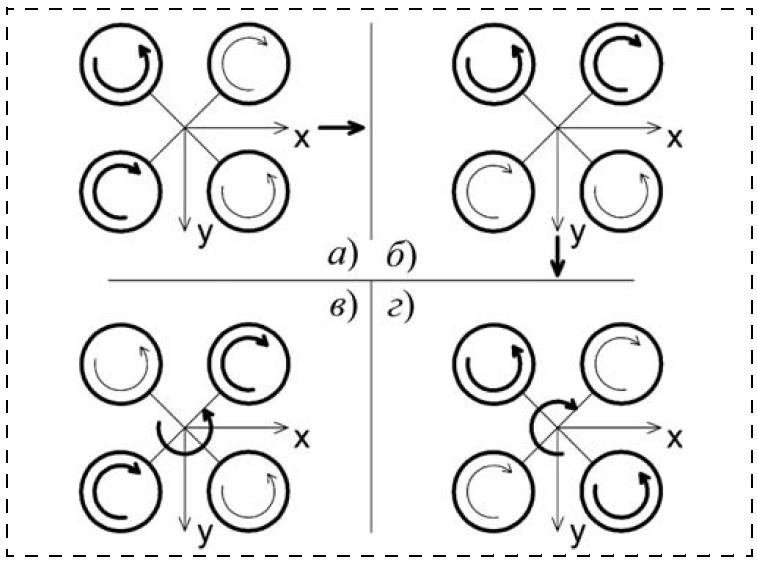
\includegraphics[width=0.7\linewidth]{others/screenshot001}
	\caption{Принцип полёта квадрокоптера}
	\label{fig:screenshot001}
\end{figure}
 
\par
Если одна пара пропеллеров, расположенных друг против друга по
диагонали, вращается по часовой стрелке, то другая пара вращается против
часовой стрелки. Дело в том, что при вращении винта возникает момент,
вращающий квадрокоптер вокруг собственной оси в обратную сторону. Если
вращать пропеллеры попарно в разные стороны, то и момент, действующий на
тело квадрокоптера и возникающий в результате вращения пары пропеллеров
по часовой стрелке, будет компенсироваться моментом, возникающим в
результате вращения пары пропеллеров против часовой стрелки. В вертолетах
эту функцию выполняет хвостовой винт, компенсирующий момент,
возникающий в результате вращения несущего винта вертолета. Вращение
вокруг собственной оси осуществляется за счет разницы скоростей вращения
между парами пропеллеров, вращающихся в разные стороны.
\subsection{Алгоритмы управления одиночным роботом}
Способ управления квадрокоптером чаще всего базируется на ПД или ПИД регуляторах, а также на линейно-квадратичных
регуляторах (ЛКР), нечетких регуляторах и нейросетевых регуляторах.
\par
ПИД-регулятор — в настоящее время наиболее часто встречающийся регулятор на технологическом производсве. Он применяется почти во всех задачах стабилизации, в частности его часто используют для стабилизации углов квадрокоптера в воздухе, для полёта по траектории и удержания позиции с помощью GPS, для удержания высоты по барометру, для стабилизации камеры в подвесе. Причиной для широкого использования служит простота построения и промышленного использования, ясность функционирования и пригодность для решения большинства практических задач.
\par
Как было упомянуто выше помимо ПИД-регуляторов существует несколько линейных регуляторов. В их числе: П-регуляторы, ПИ-регуляторы, ПД-регуляторы, И-регуляторы, Д-регулятор.
\par
Одним из минусов ПИД-регулятора является необходимость в настройке коэффициентов, которая требует  детального описания моделируемой системы. Однако, достаточно полно смоделировать такую сложную систему как квадрокоптер — не всегда возможно. По этой причине для задачи вычисления коэффициентов ПИД-регулятора используют нейросети. Совокупность этих двух подходов называют нейросетевым регулятором. \par
\subsection{Групповое управление}
Группой роботов называется совокупность
некоторого числа однотипных или разнотипных роботов, объединенных
общей целевой задачей. Для решения задачи, поставленной перед группой роботов или еѐ
частью, в недетерминированной среде каждый из роботов выполняет ряд
действий, направленных на решение общей задачи. Эти действия 
должны быть определенным образом скоординированы, согласованы по
времени, а часто и в пространстве. Таким образом, возникает задача
управления группой роботов, которая заключается либо в реализации
заранее найденной последовательности действий роботов группы, либо в
оперативном
формировании
последовательности
действий
самими
и
роботами
одновременной
или
рациональной
последующей
реализации этой последовательности. Имея в виду данную формулировку задачи группового управления,
предполагается,
что
рассматриваемые
далее
группы
состоят
из интеллектуальных роботов, то есть снабжены достаточно мощным вычислительным комплексом.
\par
Управление роботами группы осуществляется системой группового
управления роботами которая может основываться на одной из следующих стратегий:
\begin{itemize}
	\item Централизованная стратегия управления
	\item Децентрализованная стратегия управления
	\item Гибридная стратегия управления
\end{itemize}
\subsubsection{Централизованное управление}
При
реализации
методов
централизованного управления группа роботов имеет центральное управляющее устройство,
вычислительный комплекс которого является технической базой системы
управления. Управляющее устройство формирует и распределяет действия роботов группы по информационным каналам. При такой стратегии роботы-исполнители, фактически, решают лишь локальные
задачи управления, поэтому могут иметь простые вычислительные комплексы, а значит и небольшие размеры. Однако подход требует наличия надёжного канала связи между управляющим устройством роботами, при потере которого система полностью выходит из строя, равно как и при поломке управляющего устройства. \par
Централизованные стратегии разделяют на:
\begin{itemize}
	\item Единоначальное управление
	\item Иерархическое управление
\end{itemize}
Под единоначальным управлением подразумевается как расположение центрального устройства управления на пульте управления оператора (рис. \ref{fig:centr-platoon-controll}), так и использование в качестве центарального устройства управления одного из роботов группы (рис. \ref{fig:centr-platoon-agent}). 
\begin{figure}[!htbp]
	\centering
	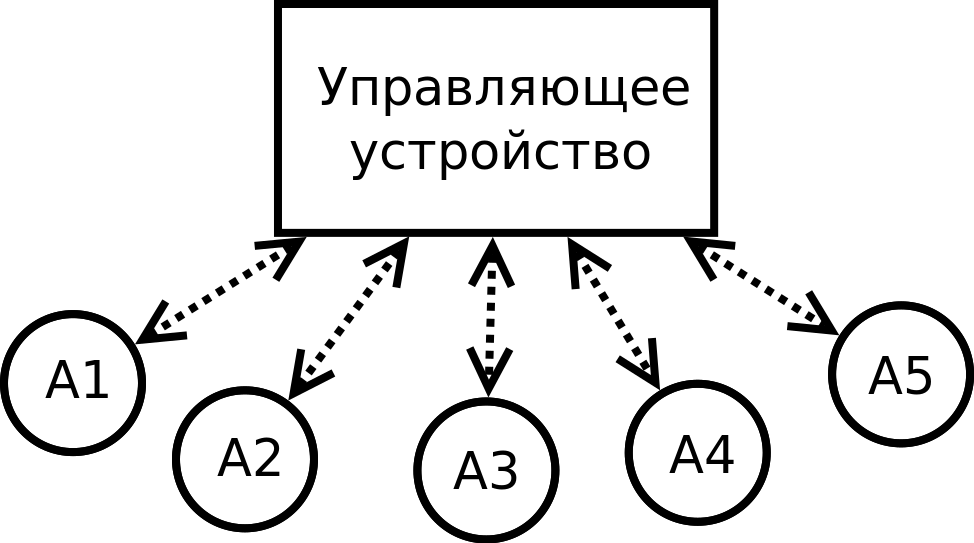
\includegraphics[width=0.7\linewidth]{others/centr-platoon-controll}
	\caption{Схема взаимодействия роботов-исполнителей $A_1$ ... $A_5$ и центрального управляющего устройства при единноначальной стратегии управления}
	\label{fig:centr-platoon-controll}
\end{figure}
\begin{figure}[!htbp]
	\centering
	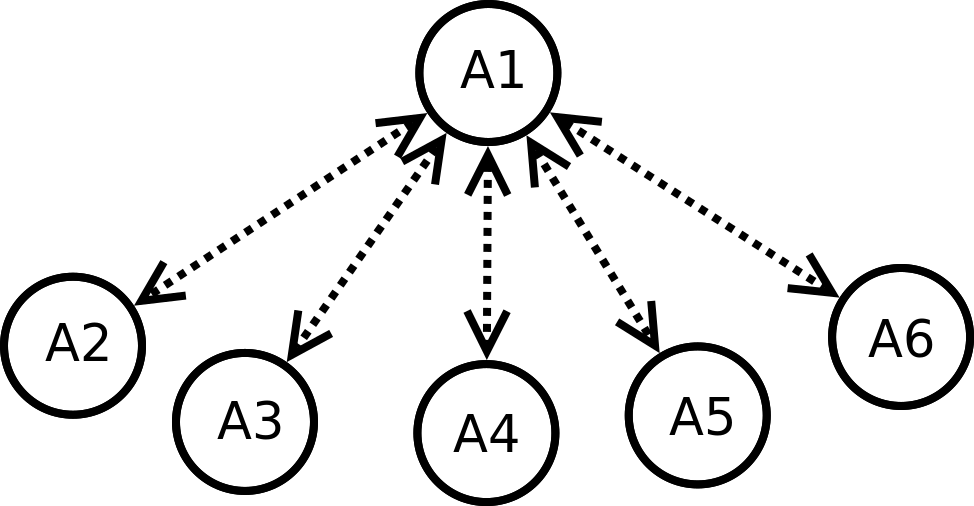
\includegraphics[width=0.7\linewidth]{others/centr-platoon-agent}
	\caption{Схема взаимодействия роботов-исполнителей $A_2$ ... $A_6$ и робота-лидера $A_1$ при единноначальной стратегии управления}
	\label{fig:centr-platoon-agent}
\end{figure}
Подход с использованием одного из агентов в качестве управляющего устройства позволяет группе дистанцироваться от исходной точки на большее расстояние, так как связи с "базой" не требуется. Однако, грузоподъёмность агента-лидера ограничивает его максимальную вычислительную мощность, а значит и сложность выполняемой задачи. \par
Так же недостатком единоначальой стратегии управления можно назвать ограниченную масштабируемость группы: одно вычислительное устройство не может справиться со сколь-угодно большим количесвом вычислений, необходимых для управления произвольным числом агентов-исполнителей. \par
Одним из выходов является применение иерархических стратегий управления (рис \ref{fig:centr-platoon}), при которых группа роботов делится на подгруппы, каждая из которых имеет своего лидера, а лидеры, в свою очередь, управляются центральным устройствоим управления (или роботом с устройством управления на борту). \par
\begin{figure}[!htbp]
	\centering
	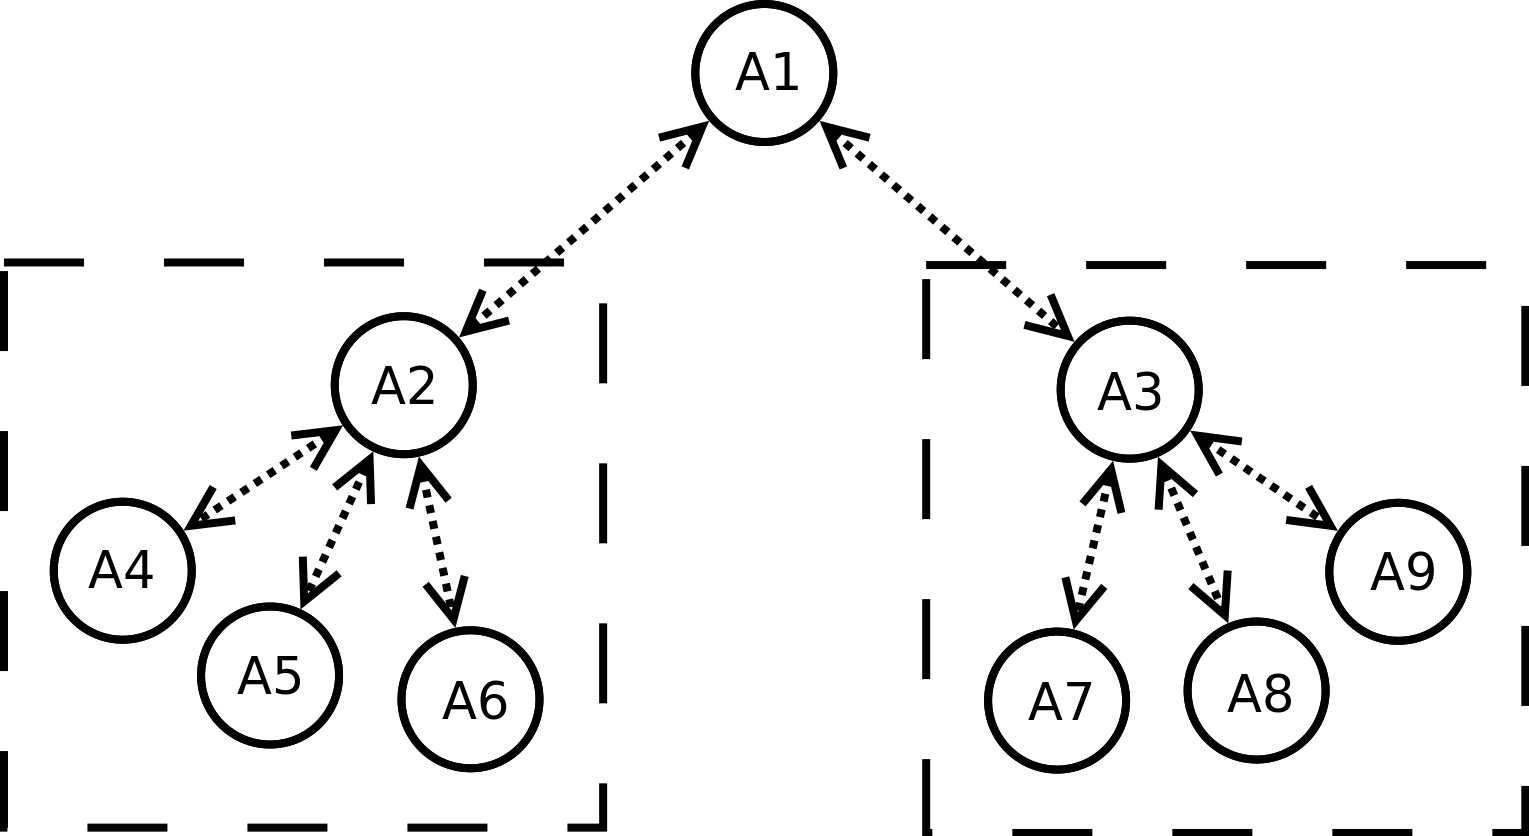
\includegraphics[width=0.9\linewidth]{others/centr-platoon}
	\caption{Схема взаимодействия лидера $A_1$, лидеров подгрупп $A_2$ и $A_3$ и роботов-исполнителей $A_4$ ... $A_9$ при иерархической стратегии управления}
	\label{fig:centr-platoon}
\end{figure}
Однако, и при таком формировании стратегии управления надёжность по прежнему низка. Отказ лидера-подгруппы приведёт к отказу всех подконтрольных роботов, а выход из строя лидера — к срыву выполняемой задачи.
\subsubsection{Децентрализованное управление}
Децентрализованная стратегия –подразумевает отсутствие в системе
единого управляющего центра формирования координационных команд, а
каждый агент независимо принимает решение о своих действиях, стремясь
принести пользу для достижения групповой цели. Такая стратегия управления
группой масштабируема и имеет высокую надежность, но сложна в
алгоритмизации. \par
Децентрализованное управление по характеру взаимодействия между агентами обычно делят на следующие типы: \par
\begin{itemize}
	\item Коллективное управление
	\item Стайное управление
	\item Роевое управление
\end{itemize}
\smallskip
При коллективной стратегии управления (рис. \ref{fig:decen-platoon-collective}) каждый робот группы передаёт  собранные им данные об окружающей среде, о своём состоянии, о его представлении обо всех остальных роботах группы в общий канал связи таким образом, что эта информация доступна всем остальным роботам группы. С помощью информации в канале каждый робот самостоятельно оценивает обстановку и принимает решение о своих дальнейших действиях. \par
\begin{figure}[!htbp]
	\centering
	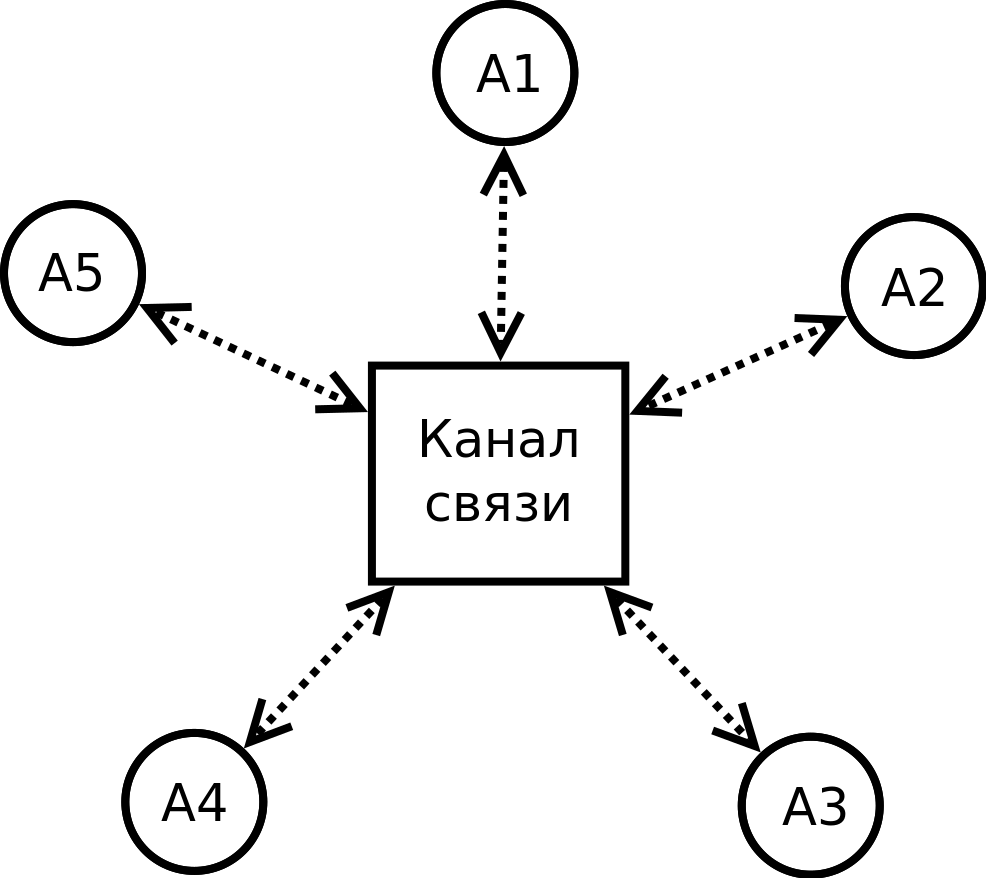
\includegraphics[width=0.6\linewidth]{others/decen-platoon-collective2}
	\caption{Схема взаимодействия равнозначных агентов $A_1$...$A_5$ через общий канал связи}
	\label{fig:decen-platoon-collective}
\end{figure}
Группа сохраняет работоспособность в случае выхода из строя одного из роботов, но требует, чтобы все агенты находились друг от друга на расстоянии не выше, чем максимальная дальность работы приборов связи, для поддержки канала. Если между двумя агентами будет превышено это расстояние, то они начнут работать в условиях недостаточности информации, и если эту ситуацию не учесть заранее, то выполнение групповой задачи может быть нарушено. Аппаратные требования к агентам достаточно высоки, однако на сегодняшний день вычислительная техника среднего ценового сегмента имеет достато мощности, чтобы справиться с предполагаемыми нагрузками. \par
Нагрузка на канал
связи между роботами возрастает прямо пропорционально увеличению численности группы роботов. Также возрастает нагрузка на бортовые вычислительные устройства роботов, так как им необходимо обрабатывать принятую информацию. Хотя
верхний предел допустимой численности группы у коллективных методов управления в среднем выше, чем у централизованных, масштабируемость этих методов оставляет желать лучшего. \par
\bigskip
При стайных стратегиях управления (рис. \ref{fig:decen-platoon-roe}) выделенный канал связи для обмена информацией между роботами отсутствует, каждый робот собирает информацию об окружающей среде и местоположениях остальных роботов самостоятельно и так же самостоятельно принимает решение о своих последующих действиях с тем расчетом, чтобы внести свой вклад в выполнение групповой задачи. Коммуникация между роботами, фактически отсутствует, что ограничивает спектр приложений до задач, которые могут легко распараллеливаться на независимые несвязные подзадачи. \par
\begin{figure}[!htbp]
	\centering
	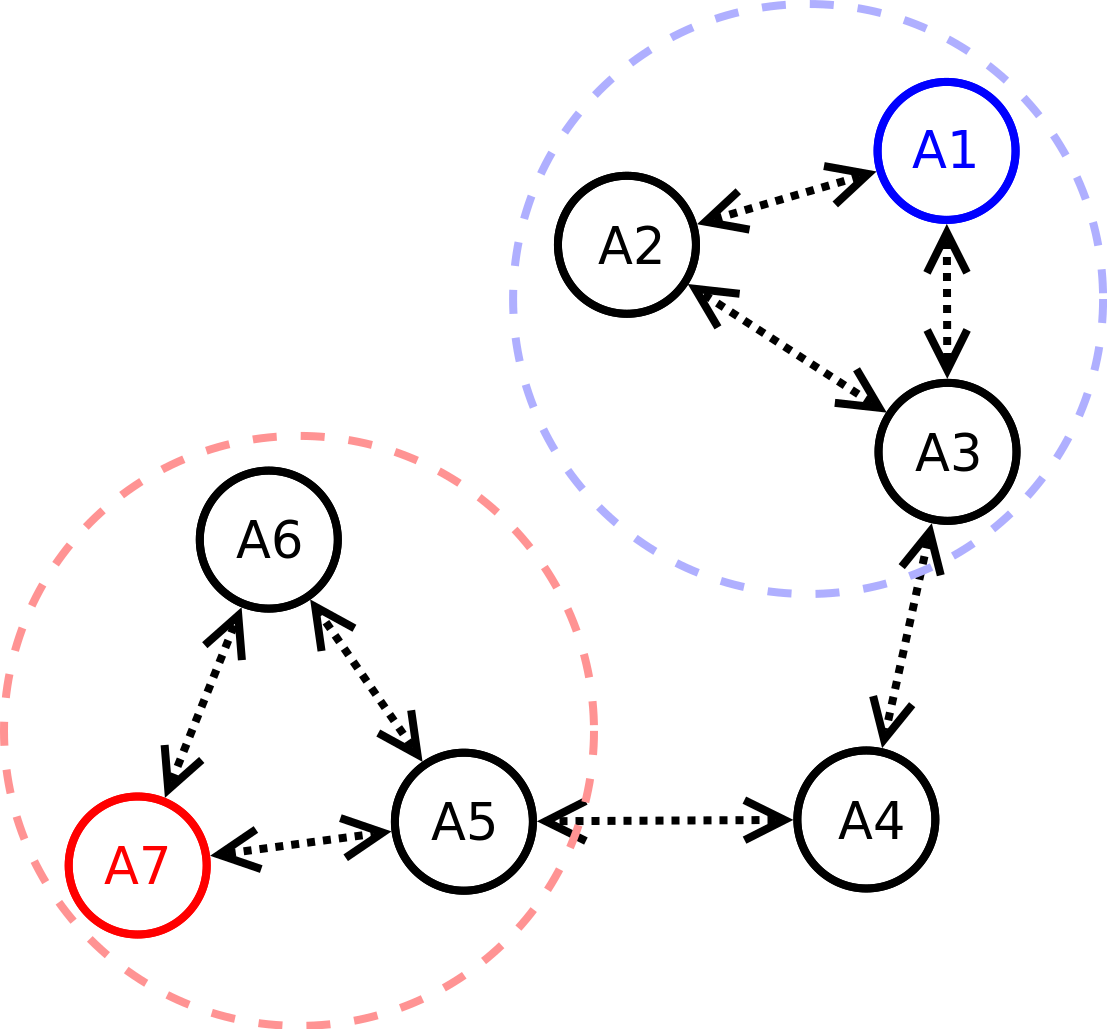
\includegraphics[width=0.55\linewidth]{others/decen-platoon-roe}
	\caption{Группа агентов $A_1$...$A_7$ с изображенными для агентов $A_1$ и $A_7$ зонами радиовидимости}
	\label{fig:decen-platoon-roe}
\end{figure}

\bigskip
При роевой стратегии управления каждый робот
группы взаимодействует лишь с некоторыми
соседними роботами, попадающими в зону видимости, ограниченную дальностью действия
его телекоммуникационных приборов (либо ограниченную искусственно). Каждый робот
самостоятельно принимает решение о дальнейших действиях, опираясь на простые локальные правила (simple rules, local rules). Роботу
доступна та информация об окружающей среде, которую он собрал самостоятельно, а также
та информация об окружающей среде и о состоянии некоторых роботов группы, которую
ему передали соседние роботы. Собранную информацию об окружающей среде, а также
о собственном состоянии робот передает в канал связи. Эта информация становится доступна тем роботам, в зону видимости которых попадает этот робот (в случае одинаковых по радиусу зон видимости — это те же соседние
роботы). Благодаря такому подходу роботы получают больше информации об окружающей
среде, чем при стайных стратегиях управления,
при этом доступная им информация касается
окружающей их области, т. е. наиболее актуальна. При этом сохраняется масштабируемость — увеличение численности группы не
приводит к увеличению нагрузки на бортовые
вычислительные устройства. \par
\subsection{Управление строем}
Частным случаем группового управления группой является строевая задача. В ней, помимо достижения поставленной цели от группы агентов требуется поддержание упорядоченного рисунка в течение всего времени выполнения задачи. \par 
Строй БПЛА может применяться для видеомониторинга местности, формирования фазированных антенных решеток и ряда других задач. Так же при задании специфического рисунка строя можно добиться снижения энергозатрат на движение некоторых роботов. Например, можно добиться этого сформировав группу агентов в клин, аналогичный клину, который создаёт косяк перелётных птиц.
\section{Постановка задачи}
\subsection{Описание постановки}
В этой работе будет разработан алгоритм роевого управления группой роботов, объединённых в строй с произвольным порядком (рисунком). Каждый робот в строю является интеллектуальным агентом, движущимся в соответствии со своим законом управления, который направлен, во-первых на то, чтобы выполнить общую задачу, а во-вторых чтобы сохранить исходную структуру строя. В качестве задачи, которая будет выполняться строем была выбрана задача движения по произвольной траектории с задаваемой скоростою. \par
Для взаимозаменяемости требования с аппаратной точки зрения ко всем агентам однинаковые, однако программно в каждый момент времени агент будет принадлежать одному из двух классов:
\begin{itemize}
	\item Мастер — агент, задача которого отрабатывать движение по траектории и быть главным ориентиром для всех остальных агентов.
	\item Миньон — агент, задача которого сохранять своё местоположение относительно других участников группы, тем самым сохраняя структуру строя
\end{itemize}
\par
Моделирование в работе будет проводиться в горизонтальной 2D плоскости. Моделями агентов будут материальные точки с массой.
\par
Ограничения:
\begin{itemize}
	\item У каждого агента есть ограничение видимости. Если два участника строя в данный момент времени находятся вне зоны видимости друг-друга, то они не могут напрямую обмениваться информацией
	\item Максимальное по модулью управляющее воздействие ограничено
	\item Агенты передают друг-другу информацию только о своих координатах
\end{itemize}
Основные требования к решению:
\begin{itemize}
	\item Без возмущений строй должен отрабатывать заданную траекторию с малыми погрешностями
	\item При малых возмущениях каждый отдельно взятый агент не должен существенно отколняться от своей позиции в строю. Строй в целом должен по прежнему выполнять задачу, с погрешностями соразмерными возмущениям
	\item При краткосрочных больших возмущениях, даже если строй потерял целостность, он должен самовосстанавливаться и продолжать выполнение задачи
	\item При выходе из строя одного или нескольких агентов строй должен переформироваться так, чтобы сохранить исходный рисунок. Строй должен быть устойчив как к отказу мастера, так и к отказу любого из миньонов
\end{itemize}
\subsection{Формальная постановка}
Вектор состояния каждого агента в горизонтальной плоскости $xy$:
$$ X = 
\begin{bmatrix}
	x_1 \\
	x_2 \\
	x_3 \\
	x_4
\end{bmatrix} ,
$$
где $x_1 = x$, $x_2 = \dot{x}$, $x_3 = y$, $x_4 = \dot{y}$. Тогда закон движения:
$$\dot{X} = AX + BU$$

\section{Алгоритм управления}
В предлагаемом мной алгоритме управления агентов можно разделить на два класса:
\begin{itemize}
	\item мастер — агент, который отрабатывает движение по траектории
	\item миньон — поддерживает своё местоположение в строю
\end{itemize}
Закон управления для этих двух типов агентов задаётся по-разному.
\subsection{Мастер}
Мастером является агент, для которого желаемый закон движения $S_d$ задаётся оператором извне: это может быть записанная в память агента траектория, целевая позиция или скорость. \par
Фактически, этот агент ничего не знает о существовании других агентов в строю (миньонов). Его задача — выполнение поставленного закона движения, поэтому закон управления зависит только от закона движения:
$$ \vec{u} = \vec{u}(S_d)$$
Рассмотрим конкретный закон управления $\vec{u}_{tr}$: движение по некоторой траектории $\vec{tr}(t)$:
$$ \vec{u}_{tr} = \vec{u}_{along} + \vec{u}_{across} $$
Закон управления состоит из двух частей. Первая $\vec{u}_{along}$ отвечает за усилие вдоль траектории, вторая $\vec{u}_{across}$ — поперёк. Направлением для $\vec{u}_{along}$ служит направление вектора между текущим положением агента и следующей точкой траектории.
\begin{center}{\textit{ (Тут будет более подробно о том, как вычисляется следующая точка траектории, о алгоритмах управления на PD регуляторах, которые используются как в $\vec{u}_{along}$, так и в $\vec{u}_{across}$)}}
\end{center}
Пример движения мастера по траектории, задаваемой параметрическим уравнением, где $s$ — параметр: $s \in [0, 5000]$.
$$x(s) = 300 \cdot \cos(\frac{s}{300}); \ y(s) = s$$

\begin{figure}[!htbp]
	\centering
	\begin{subfigure}{.5\textwidth}
		\centering
		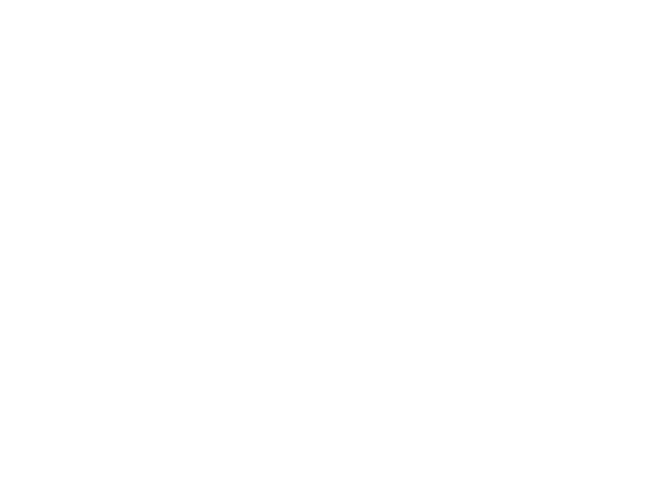
\includegraphics[width=1\linewidth]{master-trajectory-0}
		\caption{Исходная траектория и след от движения}
		\label{fig:sub1}
	\end{subfigure}%
	\begin{subfigure}{.5\textwidth}
		\centering
		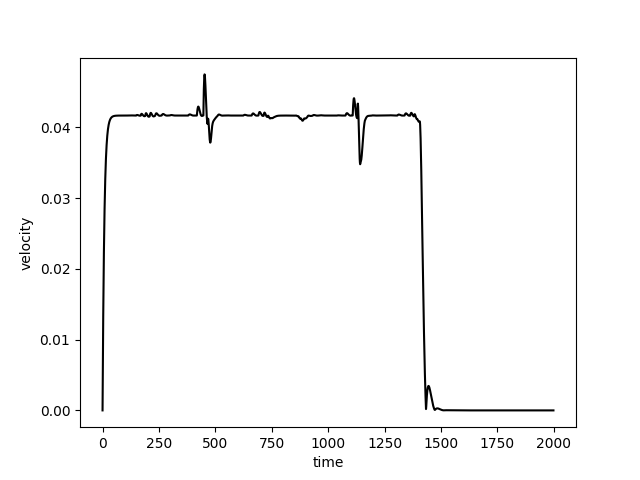
\includegraphics[width=1\linewidth]{master-trajectory-0-velocity}
		\caption{Скорость движения мастера}
		\label{fig:sub2}
	\end{subfigure}
	\caption{Движение мастера по заданной траектории с заданной скоростью $\upsilon_{desired} = 20 \frac{\text{м}}{\text{с}}$. Расстояния на рисунках задаются в метрах, время в секундах, скорость в $\frac{\text{м}}{\text{с}}$}.
	\label{fig:test}
\end{figure}
\subsubsection{Оценка движения мастера по траектории}
Агент преодолел заданную траекторию за $t = 331 \text{с}$. \\
Проеденное расстояние:
$$ S = \int_{0}^{5000} \sqrt{x'^2(s) + y'^2(s)} \ ds \approx 6051 \text{м} $$ \\
Средняя скорость $\upsilon_{av} = 18.3  \frac{\text{м}}{\text{с}}$. \\
Стационарным режимом движения можно назвать режим, при котором скорость агента колеблется в пределах между $18.8\frac{\text{м}}{\text{с}}$ и $21.5\frac{\text{м}}{\text{с}}$ (рис. \ref{fig:test}b). Более подробно скорость мастера в стационарном режиме можно увидеть на рис. \ref{fig:errors-master}a \\

\begin{figure}[!htbp]
	\centering
	\begin{subfigure}{.5\textwidth}
		\centering
		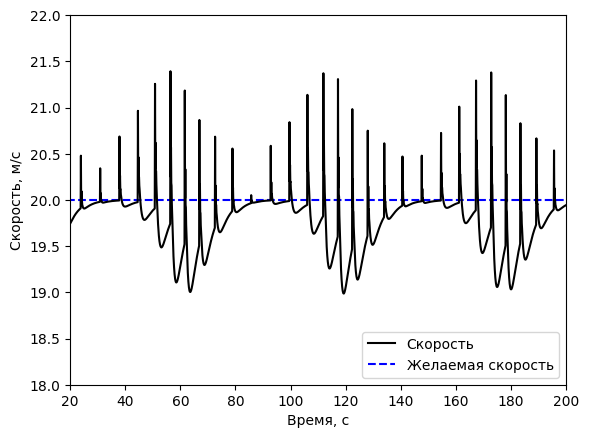
\includegraphics[width=1\linewidth]{master-trajectory-1-velocity.png}
		\caption{Скорость мастера в стационарном режиме}
		\label{fig:error-master-1}
	\end{subfigure}%
	\begin{subfigure}{.5\textwidth}
		\centering
		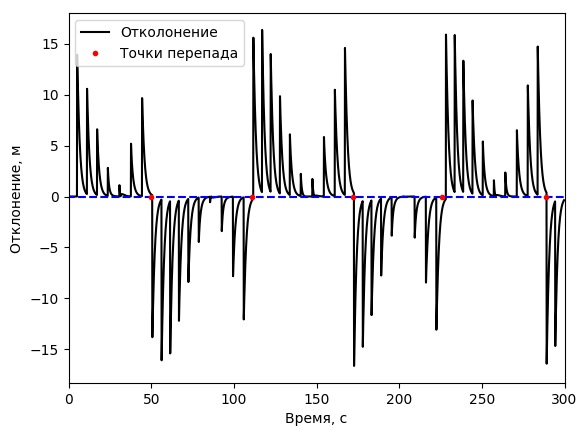
\includegraphics[width=1\linewidth]{master-trajectory-error.png}
		\caption{Отклонения мастера от траектории}
		\label{fig:error-master-2}
	\end{subfigure}
	\caption{Иллюстрация отклонений от желаемого закона движения}.
	\label{fig:errors-master}
\end{figure}
Отклонения агента от заданной траектории представлены на рис. \ref{fig:errors-master}b. Выше нуля — отклонения от траектории вправо, ниже нуля — влево. Максимальное отклонение составляет примерно 15 м. \par
Резкие перепады на графике, обозначенные как точки перепада объясняются тем, что в этих точках у траектории изменяется знак первой производной, а агент, всегда остающийся на внутренней части траектории резко оказывается на внешней. Проверим это утверждение. Заданное выше параметрическое уравнение фактически является уравнением $$x = 300 \cdot \cos(\frac{y}{300})$$
Равенство нулю первой производной:
$$\sin(\frac{y}{300}) = 0 \Rightarrow y = 300 \pi n$$
Найдём первые 5 точек траектории, в которой происходит смена знака второй производной: $$M = \Big\{(-300; \ 942), \ (300; \ 1885), \ (-300; \ 2827), \ (300; \ 3770), \ (-300; \ 4712)\Big\}$$
Найдём моменты времени, в которые эти точки будут достигнуты агентом:
$$\hat{L_t} = \Big\{ 61c, \ 118c, \ 177c, \ 234c, \ 292c \Big\}$$
Реальные же моменты времени, в которые просходит резкое изменение величины отклонения от траектории:
$${L_t} = \Big\{ 50c, \ 110c, \ 172c, \ 226c, \ 289c \Big\}$$
То есть, изменение стороны относительно линии траектории по которой движется агент изменяется незадолго до того, как будет изменён знак первой производной траектории. Эта закономерность так же наблюдается на рис. \ref{fig:master-trajectory-changes-2}. \par
\begin{figure}[!htbp]
	\centering
	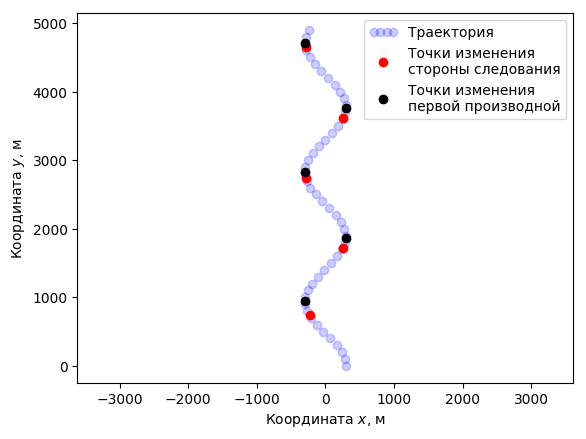
\includegraphics[width=0.5\linewidth]{master-trajectory-changes-2}
	\caption{Траектория с наложенными на неё точками изменения стороны следования и точками изменения знака первой производной.}
	\label{fig:master-trajectory-changes-2}
\end{figure}

\begin{center}{\textit{ (Тут будет исседование устойчивости алгоритма к случайным возмущениям)}}
\end{center}

\subsubsection{Выводы}
Движение мастера по траектории является точным и предсказуемым. Данный алгоритм управления по траектории с задаваемой скоростью является пригодным для применения.

\pagebreak


\subsection{Миньон} \label{minion-section}
Миньон является ведомым агентом, во время движения он никак не использует информацию о траектории движения. Всё, что использует миньон $i$ — это положения доступных для него агентов лидеров $L_k$. Относительно них миньон выстраивает свой закон управления $\vec{u_{m}}$: 
$$\vec{u_{m}} = \vec{u_{m}}(L_k)$$
\par
Более подробно об агентах-лидерах будет сказано в гл. \ref{platoon-section}, а пока о них можно думать просто как о постоянно обновляемой точке, относительно которой агент строит некую другую точку, в которую стремится попасть. Эта точка будет называться виртуальным лидером $L^v$. Точка виртуального лидера своя у каждого миньона и зависит только от реального положения агентов-лидеров $L$.\par
Пусть, есть миньон с координатами $\vec{A_1}$ и виртуальным лидером в точке $\vec{L_1^v}$. Первый закон управления, который приходит на ум может выглядеть следующим обаразом:
\begin{equation} \label{eq:wrong-controll-minion}
\vec{u_{m}}(t) = S \cdot P \text{, где } S = \big{(}\vec{L_1^v} - \vec{A_1} \big{)}
\end{equation}
\par
Суть такого закона управления в том, что воздействие осуществляется в направлении виртуального лидера с усилием пропорциональным расстоянию между текущей координатой и координатой виртуального лидера. Коэффициент $P$ — пропорциональная составляющая PID регулятора. \par
Однако, такой закон управления не выдерживает некоторых испытаний.
\subsubsection{Воздействие на агента-лидера функцией Хевисайда}
Этот численный эксперимент заключается в следующем: есть пара агентов — миньон и его агент-лидер. На агента-лидера воздействует сила по закону Хевисайда, то есть, фактически, после некоторого момента времени $\hat{t}$ появляется постоянное воздействие на агента-лидера. \par
Для облегчения понимания ситуации рассмотрим воздействие на примере.\par
\begin{figure}[h]
	\centering
	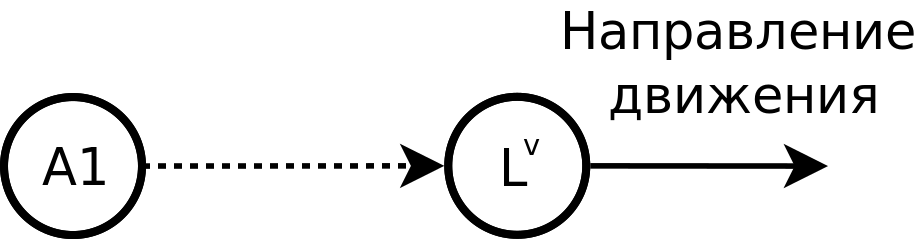
\includegraphics[width=0.4\linewidth]{minion/heviside_struct}
	\caption{}
	\label{fig:hevisidestruct}
\end{figure}
На рис. 4 изображён миньон $A_1$ и его виртуальный лидер $L^v$. На $L^v$ действует сила (распределённая как функция Хевисайда):
$$
F(t) = \begin{cases} 
1 \text{, если $t \geq 5$c} \\
0 \text{, в остальных случаях} \end{cases}
$$

Если использовать закон управления, записанный уравнением (\ref{eq:wrong-controll-minion}), то возникнет ситуация, при которой расстояние между миньоном и его виртуальным агентом будет постоянно расти. Ускорение лидера будет расти быстрее, чем ускорение миньона из-за того, что агент строит свой закон управления только на основании положения лидера, ничего не зная о его ускорении и скорости. Однако передавать эти данные от лидера к миньону может оказаться слишком накладно, т.к. придётся поддерживать более широкий канал связи.
\par
В качестве альтернативы миньон может использовать уже имеющиеся данные о положениях виртуального лидера и увеличивать управляющее воздействие, если расстояние между ним и лидером растёт $\dot{S}$. Так же для устранения статических ошибок добавляется $I$ составляющая PID регулятора.
\begin{equation} \label{eq:right-controll-minion}
\vec{u_{m}}(t) = P \cdot S  + I \cdot \int_0^t{S}dt + D \cdot \dot{S}
\end{equation}
Результаты численного моделирования с данным законом управления представлены на рисунках \ref{fig:hevisideaccelerations}, \ref{fig:hevisidevelocity}, \ref{fig:hevisidetargerr}, \ref{fig:errors-minion-heviside}.
\begin{figure}[!htbp]
	\centering
	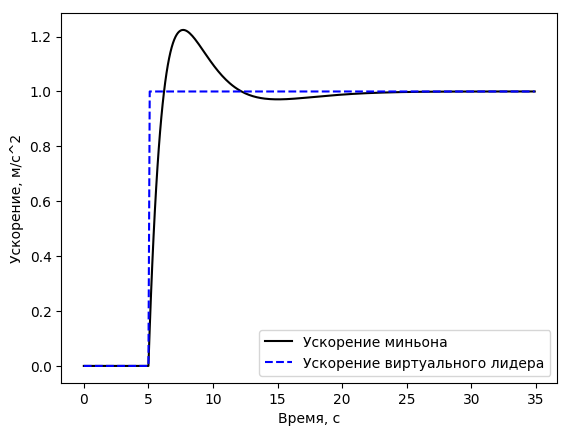
\includegraphics[width=0.6\linewidth]{minion/heviside_accelerations}
	\caption{Ускорение миньона и его виртуального лидера. Вирутальный лидер ускоряется по закону Хевисайда. Ускорение выходит на стационарный режим на 25с: через 20с. после воздействия.}
	\label{fig:hevisideaccelerations}
\end{figure}

\begin{figure}[!htbp]
	\centering
	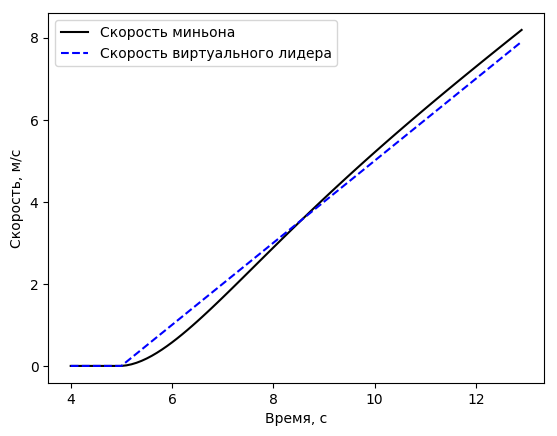
\includegraphics[width=0.6\linewidth]{minion/heviside_velocity}
	\caption{Скорость миньона и виртуального лидера}
	\label{fig:hevisidevelocity}
\end{figure}
\begin{figure}
	\centering
	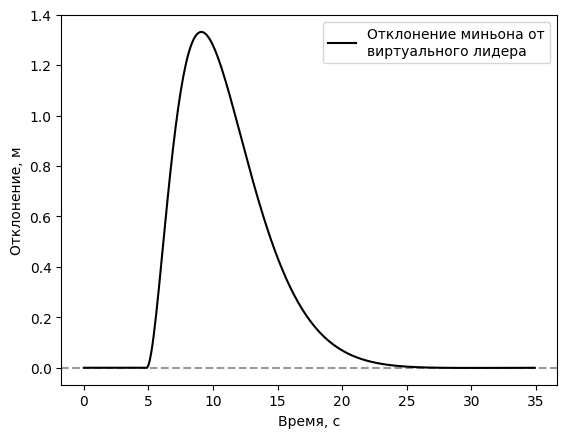
\includegraphics[width=0.6\linewidth]{minion/heviside_targerr}
	\caption{Отклонение положения миньона от его виртуального агента}
	\label{fig:hevisidetargerr}
\end{figure}




\begin{figure}[!htbp]
	\centering
	\begin{subfigure}{.5\textwidth}
	\centering
	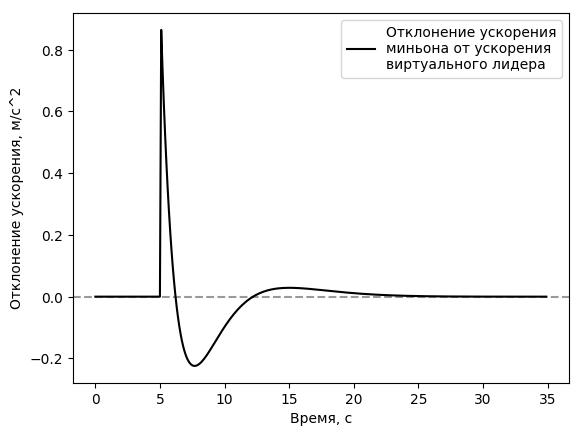
\includegraphics[width=1\linewidth]{minion/heviside_axerr}
	\caption{Отклонение ускорения}
	\label{fig:hevisideaxerr}
	\end{subfigure}%
	\begin{subfigure}{.5\textwidth}
	\centering
	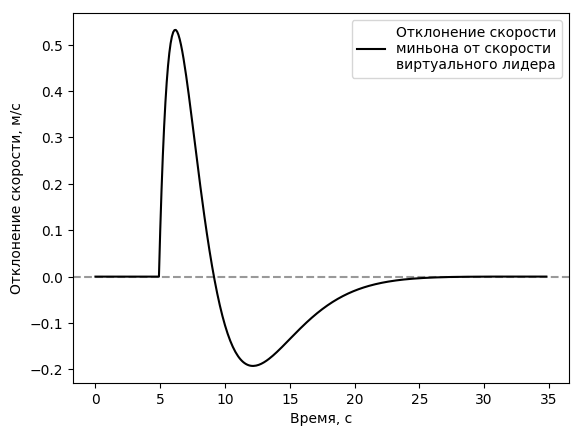
\includegraphics[width=1\linewidth]{minion/heviside_velerr}
	\caption{Отклонение скорости}
	\label{fig:hevisidevelerr}
	\end{subfigure}
	\caption{Иллюстрация отклонений от закона движения виртуального лидера. Выше нуля — значение меньше, чем у лидера, ниже нуля — выше, чем у лидера.}
	\label{fig:errors-minion-heviside}
\end{figure}
\subsubsection{Выводы}
Описанный закон управления справляется с задачей приведения миньона в точку вирутального лидера и будет использован в дальнейшем для управления строем.

\section{Строй} \label{platoon-section}

Строй представляет из себя множество агентов соединённых связями, подобно графу. Для каждого агента, не являющегося мастером (миньона) определён набор связей: каждый агент с порядковым номером $i$ связан со всеми агентами с порядковыми номерами $j: i > j$, называемыми лидерами данного миньона. Каждый агент — вершина графа, каждая связь миньон-лидер — ребро графа. Пример строя из 5-ти агентов изображён на рис.\ref{fig:wedge-platoon}. \par
\begin{figure}[!htbp]
	\centering
	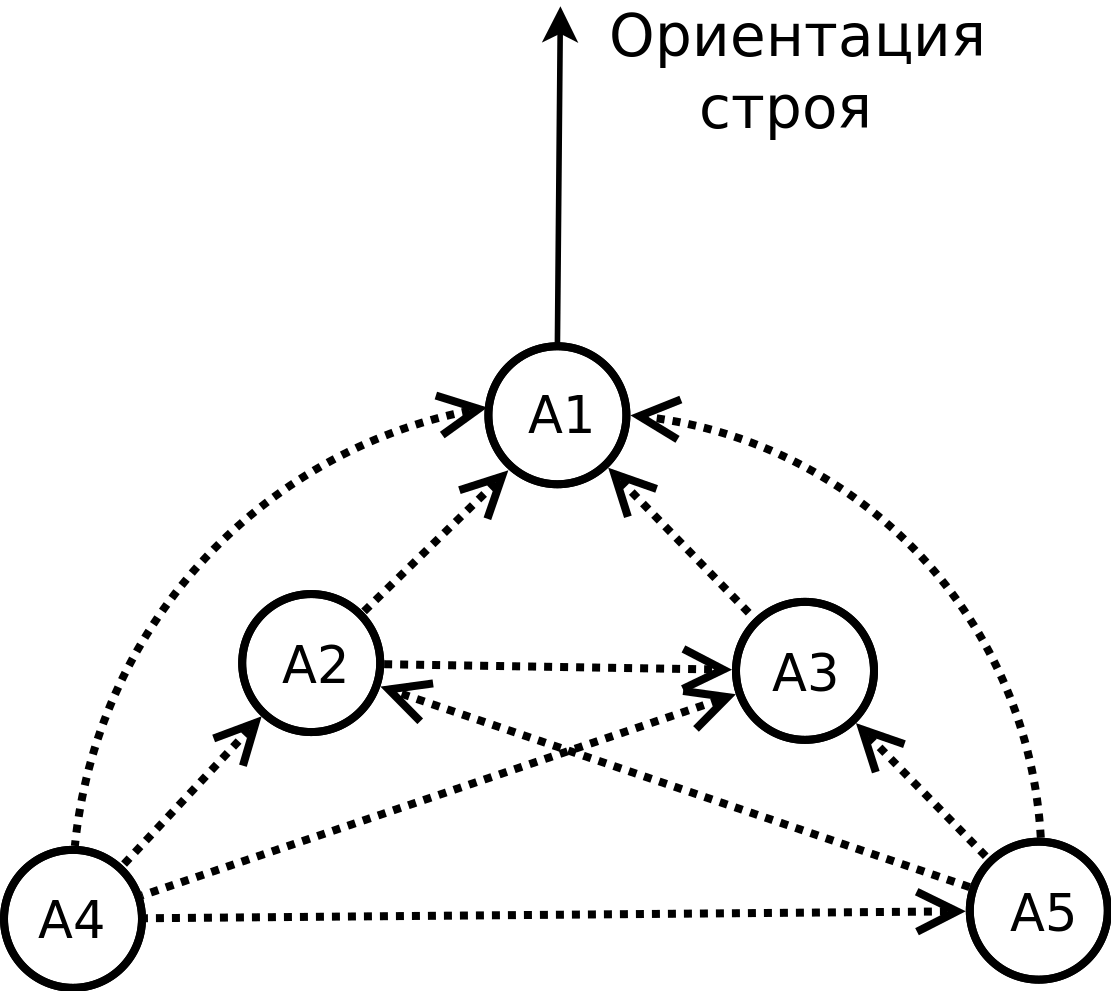
\includegraphics[width=0.5\linewidth]{platoon/wedge-platoon-full}
	\caption{Пример клиновидного строя из 5-ти агентов}
	\label{fig:wedge-platoon}
\end{figure}
Каждая связь $J_{ij}$ — это вектор в полярных координатах, у которого радиус — это расстояние от миньона $i$ до миньона лидера $j$, а угол — это угол между изначальной ориентацией строя и вектором, соединяющим миньона с его лидером. К примеру, если расстояния между каждой парой агентов равно 1м, то связи:
\begin{itemize}
	\item $J_{1j}$ — не определены ни для каких $j$: $A_1$ является мастером
	\item $J_{21} = (r=1\text{м}; \varphi=225\text{\textdegree{}})$ — для миньона $A_2$ агентом лидером является мастер $A_1$. Агенты находятся на расстоянии 1м, угол между соединяющим их вектором и вектором изначальной ориентации составляет $225 \text{\textdegree}$
	\item $J_{31}, J_{42}, J_{53}$ и т.д. — определяются аналогично
\end{itemize}
\subsection{Алгоритм поддержания строя}
В каждый момент времени положение миньона определяется положением его лидеров. Точка, в которую стремится попасть миньон называется точкой виртуального лидера. Виртуальный лидер — точка пространства, в которую стремиться попасть миньон для того, чтобы поддерживать фигуру строя. Для того, чтобы расчитать эту точку необходимо отложить вектор связи от каждого лидера этого миньона и всять центр масс от полученных точек.\par
При повороте строя местоположение каждого миньона должно измениться в соответствии с повёрнутой структурой. При повороте строя поворачивается и вектор ориентации строя, за счёт чего далее пересчитывается позиция, в которой должен находиться агент после поворота. \par
Например, на рис. \ref{fig:wedge-platoon-rotation} изображён поворот строя на угол $b$. Для того, чтобы пересчитать позицию, в которой должен находиться миньон после поворота (виртуальный лидер) необходимо для каждого доступного лидера отложить повёрнутый вектор изначальной ориентации $O_{0}$ на угол $b + \varphi$, где $\varphi$ — угол из вектора связи $J_{ij}$ миньона $i$ и выбранного лидера. Длина откладываемого вектора равна расстоянию $r$ из вектора связи. 
\par
\begin{figure}[!htbp]
	\centering
	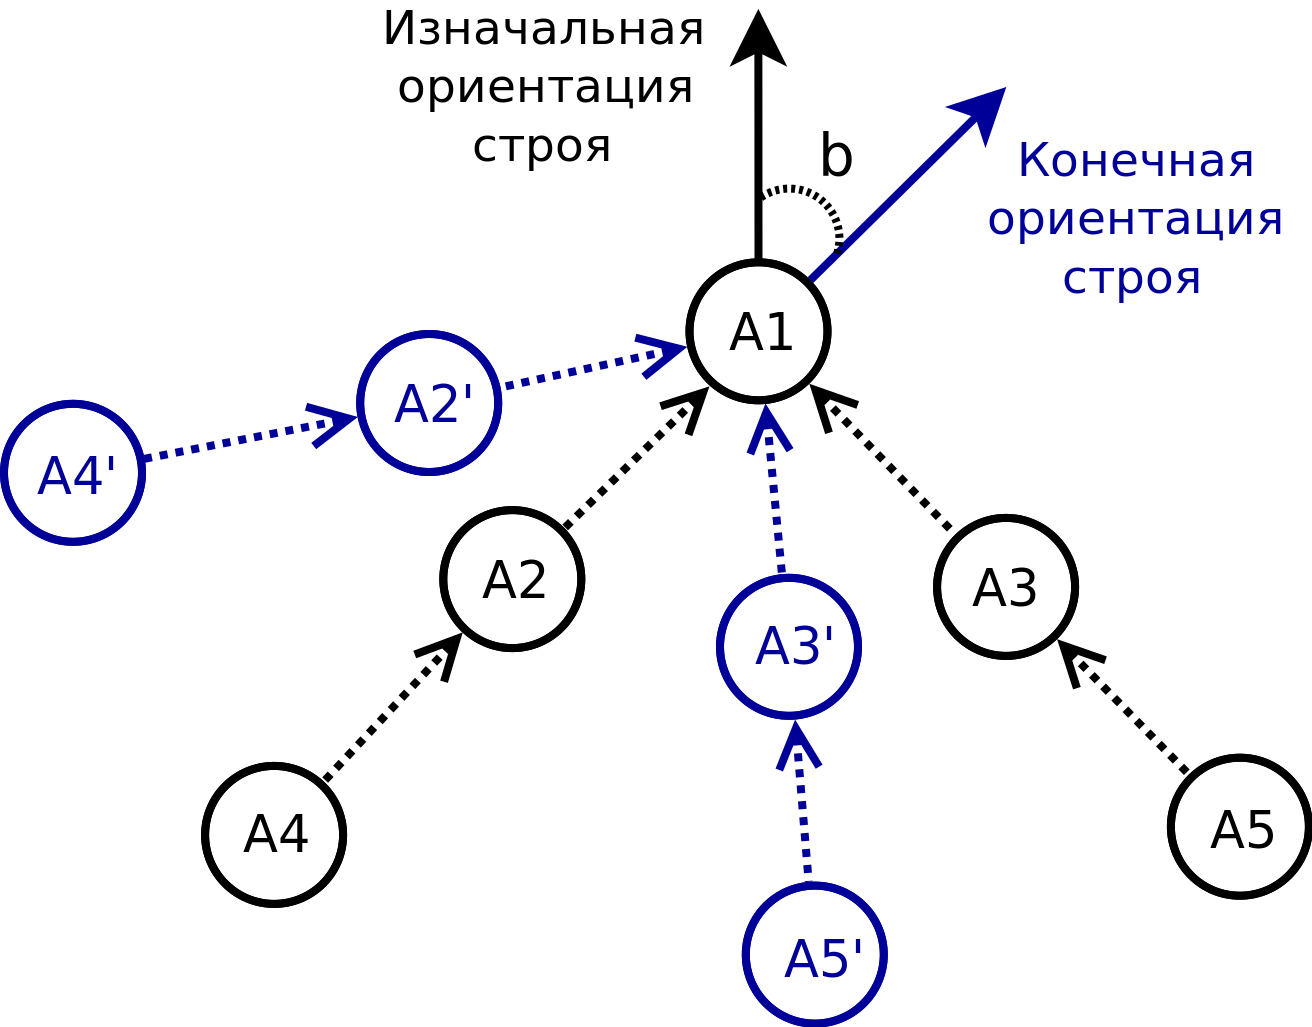
\includegraphics[width=0.5\linewidth]{platoon/wedge-platoon-rotation}
	\caption{Поворот строя на угол $b$}
	\label{fig:wedge-platoon-rotation}
\end{figure}
Рассмотрим пример того, как будет расчитан виртуальный лидер $A_5'$ для агента $A_5$ (см. рис. \ref{fig:wedge-platoon-rotation}), для которого единственным агентом-лидером в зоне видимости является $A_3$. Вектор связи между ними $J_{53} = (r_{53}; \ \varphi_{53})$. Для начала повернём вектор изначальной ориентации $O_{0}$:\par
$$\vec{O_{1}} =  \left(\begin{array}{cc} \cos{(b + \varphi_{53})} & \sin{(b + \varphi_{53})}\\ \sin{(b + \varphi_{53})} & \cos{(b + \varphi_{53})} \end{array}\right) \vec{O_{0}} $$
Теперь вдоль полученного вектора $\vec{O_1}$ необходимо отложить от позиции агента $A_3$ расстояние равное $r_{53}$:\par
$$ \vec{A'_{5}} = \vec{A_3} + \frac{\vec{O_1}}{|\vec{O_1}|} r_{53}$$ 
Если для миньона доступно больше агентов-лидеров, то виртуальный лидер будет, как уже говорилось выше, центром масс получаемых точек. Аналогичным образом каждый миньон расчитывает своего виртуального лидера и за счёт стремления в эти точки и сохраняется структура строя.\par
Резюмируя, алгоритм строевого движения заключается в том, что агенты связаны между собой. Мастер, двигаясь по траектории заставляет двигаться и всех миньонов, для которых он является лидером, а перемещение этих миньонов, приводит в движение следующий слой миньонов, для которых они являются лидерами. \par
Результат симуляции движения строя по траектории без внешних возмущений изображен на рис. \ref{fig:platoon-trajectory-0}. \par
\begin{figure}[!htbp]
	\centering
	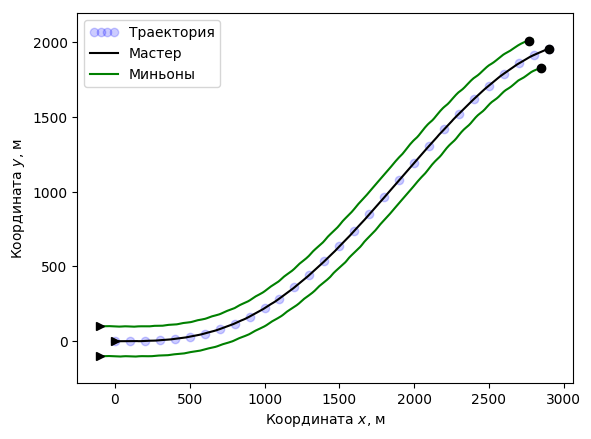
\includegraphics[width=0.7\linewidth]{platoon-trajectory-0}
	\caption{Движение строем мастера и двух миньонов}
	\label{fig:platoon-trajectory-0}
\end{figure}
Однако, более интересным является тестирование алгоритма на критические воздействия.
\subsection{Робастность алгоритма}
В этой главе будут рассмотрены некоторые сценарии воздействия на строй, дополненные описанием используемых возможностей алгоритма, не упомянутых ранее.
\subsubsection{Отказ мастера}
При отказе мастера строй не должен потерять работоспособность. Для этого в алгоритме предусмотрена возможность смены мастера на любого из агентов в строю. Чтобы объяснить механизм обнаружения выхода из строя мастера необходимо описать некоторые, до этого момента не освещённые функциональные возможности алгоритма. \par
Перед вылетом строя каждому агенту присваивается порядковый номер, который будет определять то, на каком месте в строю будет двигаться каждый из агентов. Позднее этот параметр будет определять то, на какую позицию перейдёт каждый агент, если какой-то другой агент вышел из строя. Для того, чтобы отслеживать полноту строя, между агентами создаётся общий канал связи, в который каждый из них отправляет сообщение, чтобы оповестить остальных о своей работоспособности. Если какой-то агент долгое время не отправляет данных о себе в этот канал, то остальные считают его оказавшим и строй переформировывается так, чтобы заполнить вышедший элемент. \par
Из-за того, что не каждая пара агентов может общаться напрямую (из-за ограниченной зоны радиосвязи) канал связи формируется следующим образом: каждый агент отправляет в широковещательный канал информацию не только о себе самом, но и собсвенную версию жизнеспособности всех агентов. Таким образом удаётся достичь того, что если между парой агентов есть хотя бы косвенная связь, то они будут знать о существовании друг друга.\par
\bigskip
На рис. \ref{fig:with-crashes} изображен сценарий поочерёдного выхода из строя двух агентов. Сначала мастера, затем одного из миньонов. Так же на рисунке присутствует отклонение по начальным условиям: агенты формируют строй изначально находясь в произвольных точках. Подробнее важные области изображены на рисунках \ref{fig:with-crashes-zoom3}, \ref{fig:with-crashes-zoom1}, \ref{fig:with-crashes-zoom2}. \par
Вывод: выход мастера и одного из миньонов не оказал критического влияния на строй в целом.
\begin{figure}
	\centering
	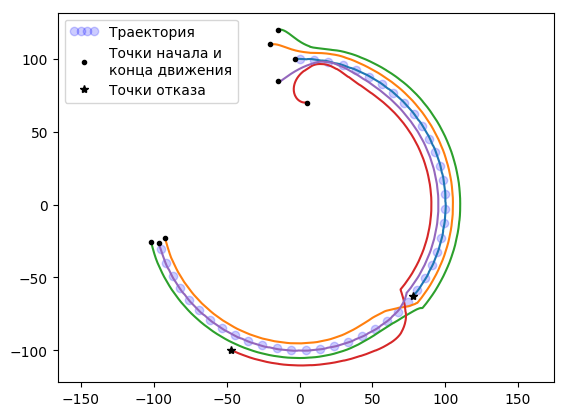
\includegraphics[width=0.7\linewidth]{platoon/with-crashes}
	\caption{Движение агентов строем с отказом двух агентов. Чёрной линеей изображён мастер. После отказа мастера происходит его смена и чёрной линеей изображается сменивший отказавшего мастер. }
	\label{fig:with-crashes}
\end{figure}
\begin{figure}
	\centering
	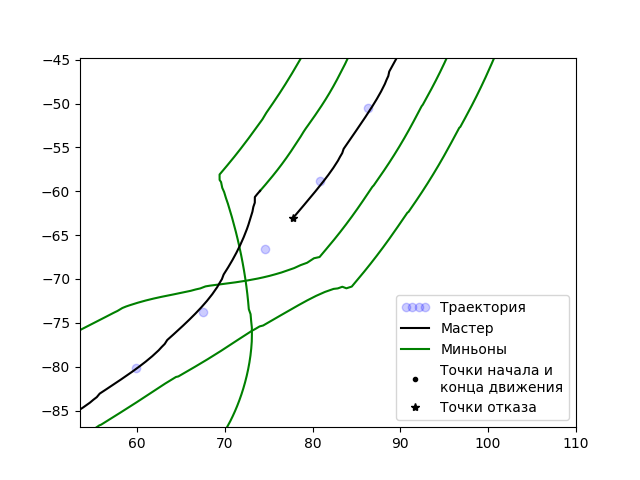
\includegraphics[width=0.7\linewidth]{platoon/with-crashes-zoom3}
	\caption{Область отказа мастера. На позицию мастера встаёт другой агент.}
	\label{fig:with-crashes-zoom3}
\end{figure}
\begin{figure}
	\centering
	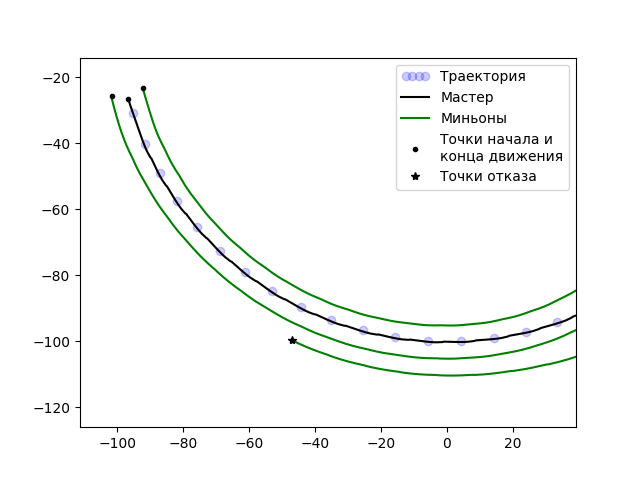
\includegraphics[width=0.7\linewidth]{platoon/with-crashes-zoom1}
	\caption{Область отказа миньона. На его позицию не встаёт никакой агент, т.к. эта позиция в строю имеет приоритет ниже, чем остальные.}
	\label{fig:with-crashes-zoom1}
\end{figure}
\begin{figure}
	\centering
	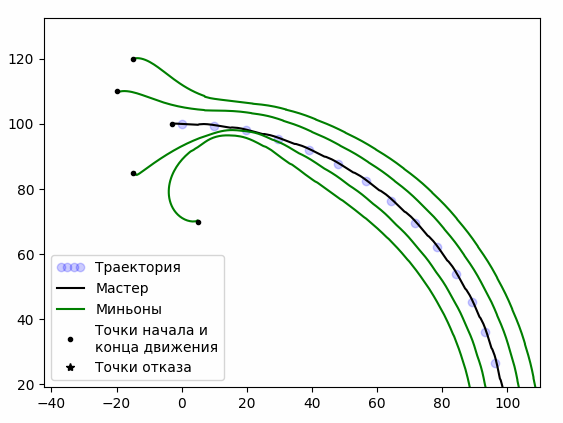
\includegraphics[width=0.7\linewidth]{platoon/with-crashes-zoom2}
	\caption{Область изначального формирование строя агентами.}
	\label{fig:with-crashes-zoom2}
\end{figure}


\subsubsection{Критически большое возмущение}
Под критически большими возмущениями имеются в виду возмущения, способные разбить строй на части. Фактически, разбить строй на части означает развести агентов в пространстве так, что одна часть не будет радиодоступна другой даже косвенно, то есть между любой парой агентов из разных частей расстояние больше чем радиус радиодоступности $R_a$. \par
Симуляция такого сценария преведена на рис \ref{fig:with-bird}. Описывается происходящее следующим образом: на двух агентов из строя в некоторый момент времени действует сильное кратковременное возмущение (рис.  \ref{fig:with-bird-zoom1}), выводящее этих агентов из зоны видимости остального строя. Далее эти два отделившихся агента формируют собственный строй (рис. \ref{fig:with-bird-to-groups}) и двигаются по заданной траектории так, будто главного строя не существует. Когда отделившийся строй попадает в зону видимости другого они сливаются в один рис. (\ref{fig:with-bird-zoom2}).
\begin{figure}
	\centering
	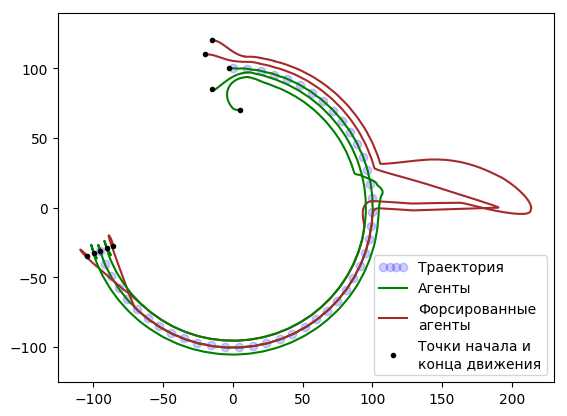
\includegraphics[width=0.7\linewidth]{platoon/with-bird}
	\caption{На двух агентов из строя кратковременно действует такая сила, что они отделяются от основного стоя}
	\label{fig:with-bird}
\end{figure}
\begin{figure}
	\centering
	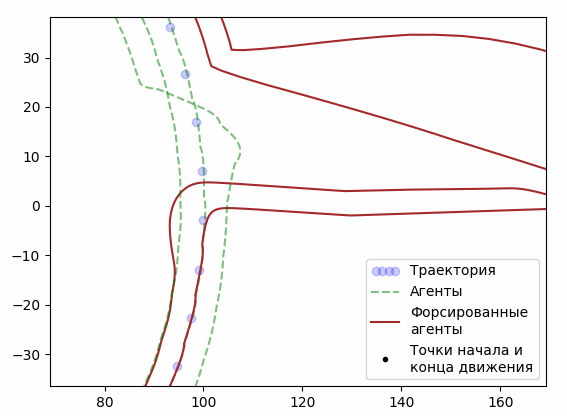
\includegraphics[width=0.7\linewidth]{platoon/with-bird-zoom1}
	\caption{Отделившиеся агенты формируют собственный строй из мастера и одного миньона и двигаются по траектории независимо от другой части изначального строя}
	\label{fig:with-bird-zoom1}
\end{figure}
\begin{figure}
	\centering
	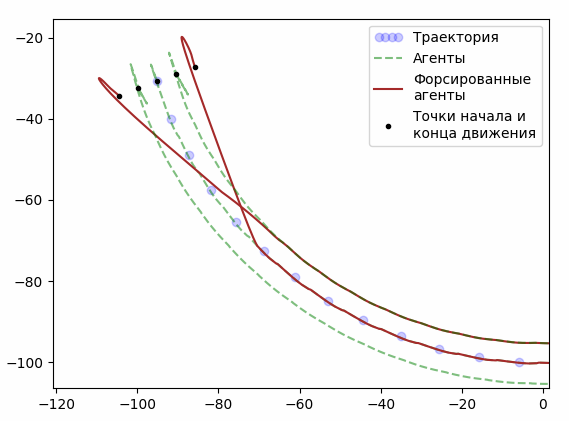
\includegraphics[width=0.7\linewidth]{platoon/with-bird-zoom2}
	\caption{При достижении отделившимся строем границы зоны видимости первого строя они сливаются в единый строй}
	\label{fig:with-bird-zoom2}
\end{figure}
\begin{figure}
	\centering
	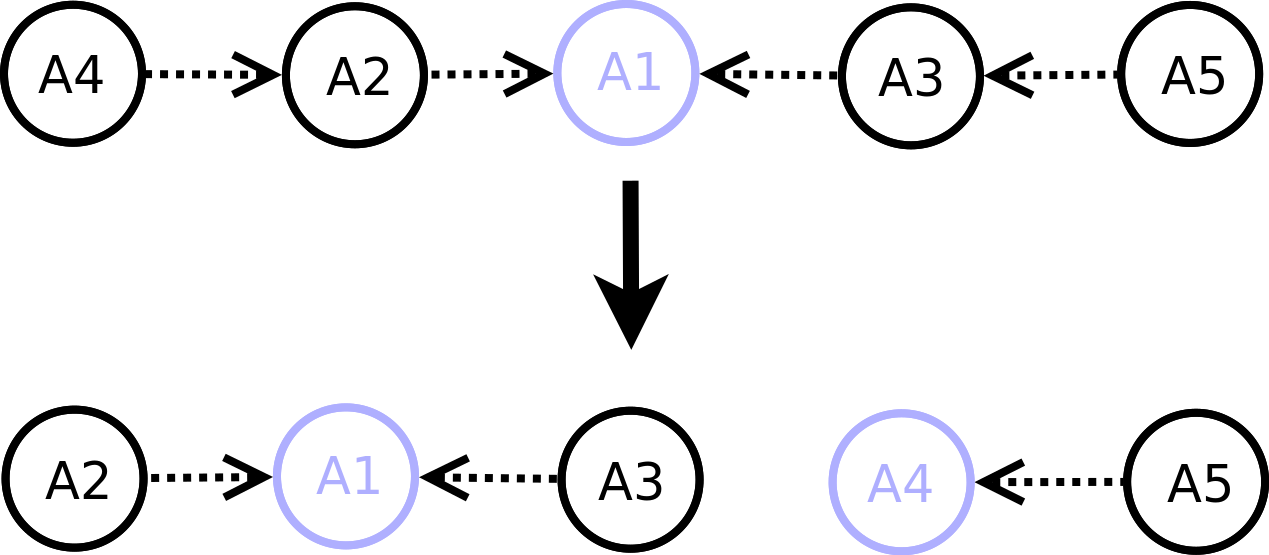
\includegraphics[width=0.7\linewidth]{platoon/with-bird-to-groups}
	\caption{Строй разбивается на две группы. В одной 3 агента, в другой 2 агента. Голубым цветом помечены мастера}
	\label{fig:with-bird-to-groups}
\end{figure}


\newpage
\addcontentsline{toc}{section}{\protect\numberline{}Список источников}%
\section*{Список литературы}
\begin{enumerate}
	\item Пшихопова В.Х. Групповое управление подвижными объектами в неопределённых средах — 2015
	\item Иванов Д.Я. Методы построения пространственных формаций в группах БПЛА типа квадрокоптеров
	\item Петров В.Ф., Барунин А.А., Терентьев А.И. Модель системы автоматического управления БПЛА
	\item Иванов Д.Я. Решение строевой задачи в группе беспилотных квадракоптеров
	\item Иванов Д.Я. Построение формаций в группах квадрокоптеров с использованием виртуального строя
	\item Каляев И.А. Самоорганизация в мультиагентных системах
	\item Галустян Н.К. Децентрализованное управление группой квадрокоптеров
	\item Амелин К.С., Антал Е.И., Васильев В.И. Адаптивное управление автономной группой летательных аппаратов
	\item Иванов Д.Я. Методы роевого интеллекта для управления группами малоразмерных беспилотных летательных аппаратов
	\item Иванов Д.Я. Использование принципов роевого интеллекта для управления целенаправленным поведением массово применяемых микророботов
	в экстремальных условиях
	\item Бесекерский В.А., Попов Е.П. Теория систем автоматического управления — 2007
	\item Морозова Н.С. Управление движением строя в мультиагентных системах — 2015
	\item Гурьянов А.Е. Моделирование управления квадрокоптером — 2014
	
\end{enumerate}

\end{document}